
\subsection{Evaluation}
\label{sec:exp:evaluation}
Table~\ref{tab:evaluation}에서 보이는 바와 같이 \sdqnname를 사용한 모델에서 마리오가 가장 먼 거리를 이동하였다.
우리의 학습 목표가 빠른 시간내에 스테이지를 감안하면 모델의 성능 평가에 시간적인 요소가 들어가야 한다.
하지만 스테이지를 클리어하지 못한 상황에서는 시간이 많이 걸리더라도 먼 거리를 이동하는 것이 바람직하다.
아쉽게도 본 실험에 사용한 모델들 (\dqnname, \sdqnname, \sadqnname) 모두 월드 1-1을 클리어하는 데까지 학습되지 못하였다.
본 실험 시간이 충분하지 못하여 각 모델들은 동일하게 10시간 동안의 학습시키고, 학습하는 중간에 마리오의 생명을 모두 소진한 경우 테스트 모드로 변환하여 마리오의 이동거리를 측정하였다.
테스트 모드에서는 학습때와는 달리 e-greedy 방법을 사용하지 않고 모델의 q-network을 사용하여 매 action을 기대되는 q값을 최대화 하도록 선택하였다.
이와 같은 실험에서 화면 분활을 통해 특정 부분에 대해 집중적으로 feature를 수집하는 \sdqnname이 마리오를 가장 먼거리로 이동시켰다.

\begin{table}[h]
\centering
\caption {
	모델별 마리오 도달거리. 월드 1-1에서만 테스트하였으며 많은 거리를 이동할 수록 숫자가 크다.
}
\label{tab:evaluation}
\begin{tabular}{llll}
\toprule
     & \dqnname  & \sdqnname & \sadqnname \\
\midrule
도달거리 & 1641 & 1784  & 1675  \\
\bottomrule
\end{tabular}
\end{table}

우리의 기대와는 달리, \sdqnname에서 attention network를 추가한 \sadqnname의 성능이 낮게 평가되었다.
이는 충분한 학습시간을 가지지 못한 우리의 상황이 학습하여야하는 파라미터의 수가 많은 \sadqnname에게 불리한 요소로 작용되었을 것으로 추측된다.


\subsection{Effectiveness of Dropout and Batch Normalization}
\label{sec:exp:dropout}
일반적인 neural network에서 dropout과 batch normalization은 모델의 overfitting을 막기위해 널리 사용되는 방법이다.
DQN기반의 모델들도 q-value function을 neural network에 기반한 함수를 사용하고 있으므로 해당 기법들이 모델의 학습에 도움이 될 것이라고 생각하였다.
\sapdqnname은 \sadqnname에서 각 CNN의 앞단에 batch normalization layer를 추가하고, action의 q값을 추론하기 직전의 MLP (Multi Layer Perceptron) 직후 30\%의 노드를 dropout시키는 dropout layer를 추가하였다.
결과적으로 \sapdqnname은 학습되는 데 실패하여 마리오의 이동거리가 40을 채 넘지 못하였다.

\begin{figure}[h]
\centering
	\begin{subfigure}[]{.48\textwidth}
		\centering
		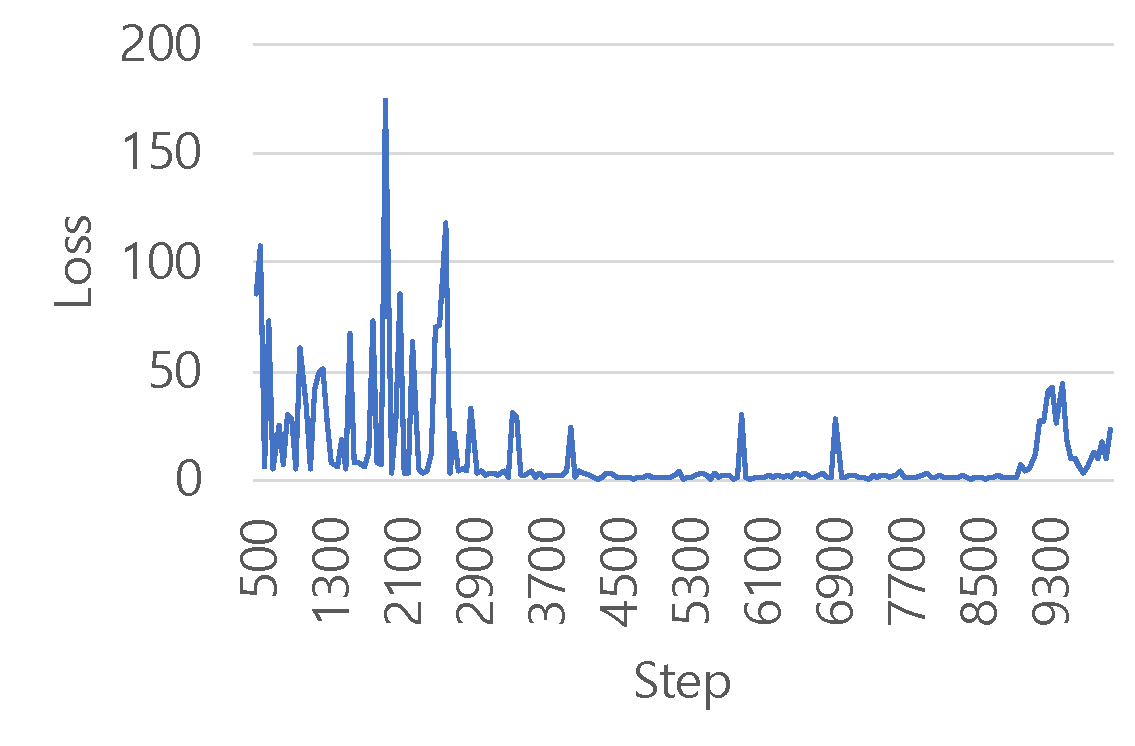
\includegraphics[width=1.\textwidth]{FIG/Loss_SADQN.pdf}
		\caption{Loss of \sadqnname}
		\label{fig:loss_sadqn}
	\end{subfigure}%
	\begin{subfigure}[]{.48\textwidth}
		\centering
		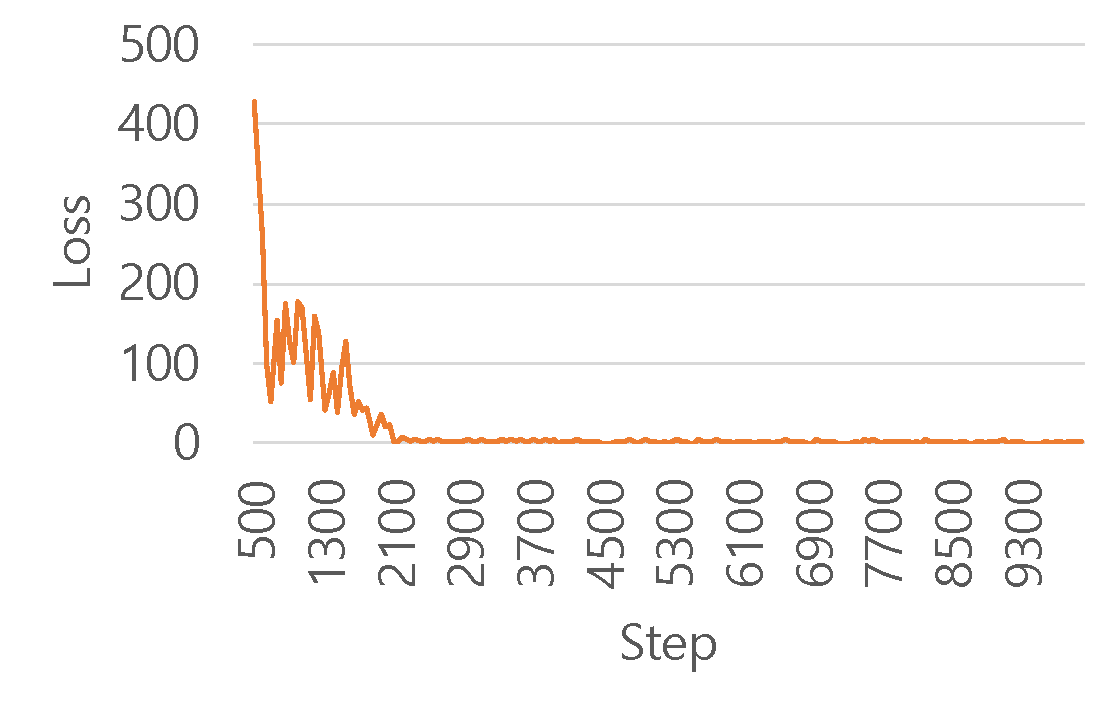
\includegraphics[width=1.\textwidth]{FIG/Loss_SAPDQN.pdf}
		\caption{Loss of \sapdqnname}
		\label{fig:loss_sapdqn}
	\end{subfigure}%
\caption{
	Step별 loss의 변화. 결과적으로 더 멀리 마리오를 이동시킨 \sadqnname의 경우 지속적으로 loss가 상승하였다가 감소하는 구간이 확인된다.
}
\label{fig:loss}
\end{figure}

Figure~\ref{fig:loss}는 step별로 \sadqnname과 \sapdqnname의 loss가 어떻게 변화하는지 보여주고 있다.
\sadqnname는 지속적으로 loss가 상승하였다가 감소하는 구간이 확인되는 반면, \sapdqnname은 loss가 한번 감소된 이후 그것을 유지하고 있다.
\sadqnname의 경우, 마리오가 더 멀리 나아가서 새로운 state를 발견하였을 때, 미지의 구간에 대한 q값 때문에 loss가 상승하였다가 이에 대한 학습이 끝나면 loss가 감소하는 것을 반복하고 있다.
반면, \sapdqnname은 마리오가 계속 시작지점에만 머물러 있기 때문에 새로운 state를 발견하지 못하고 있다.
따라서 지속적으로 발전해나가는 모델의 loss의 변화는 Figure~\ref{fig:loss_sadqn}과 같은 모양을 가지게 된다.

\subsection{Reward}
\label{sec:exp:reward}
% 이건 그냥 써본건데 혹시라도 각각의 리워드 세팅에 따라 실험한게 있다면 결과를 쓰기 위해 놔둬봤어영
Reward는 강화학습에서 모델 학습의 성공 여부를 결정짓는 중요한 요소이다.
Reward를 계산할 때 우리는 3가지 요소를 고려하였다.
첫번째 요소는 마리오의 가로 방향 이동거리인데, 좌측으로 이동할 수록 reward가 증가하고 우측으로 이동할 수록 감소한다.
두번째 요소는 마리오의 이동이 없었을 때의 패널티이다.
이때 reward를 0으로 주거나 감소시키기도 하였다.
마지막 요소는 게임의 남은 시간 (초) 이다. 남은 시간이 줄어들 수록 reward를 감소시켰다.
우리는 본 실험에서 3가지의 서로 다른 Reward를 구현하고 이전에 성능이 제일 잘 나왔던 \sadqnname으로 테스트 하였다.
3가지 Reward 세팅은 다음과 같다.
\begin{itemize}
	\item \textsc{R0}:
		가로 방향 +10 이동시 reward 5 증가 및 -10 이동시 5 감소. 이동이 없을때 패널티는 없으나, 남은 시간이 1 줄어들때 마다 reward 1 감소.
	\item \textsc{R1}:
		가로 방향 +3 이동시 reward 5 증가 및 -3 이동시 5 감소. 이동이 없을때 reward 1 감소 및 남은 시간이 1 줄어들때 마다 reward 1 감소.
	\item \textsc{R2}:
		가로 방향 +1 이동시 reward 5 증가 및 -1 이동시 5 감소. 이동이 없을때 reward 1 감소 및 남은 시간이 1 줄어들때 마다 reward 1 감소.
\end{itemize}

\begin{table}[h]
\centering
\caption {
	Reward별 \sdqnname의 마리오 도달거리.
}
\label{tab:reward}
\begin{tabular}{llll}
\toprule
     & R0  & R1 & R2 \\
\midrule
도달거리 & 1423 & 1784  & 1439  \\
\bottomrule
\end{tabular}
\end{table}

Table~\ref{tab:reward}에서 각 reward별 \sadqnname의 마리오 도달거리를 확인할 수 있다.
R1이 가장 좋은 성능을 보이고 있다.
R0의 경우에는 이동이 없을 때 패널티가 없어서 마리오가 계속 멈추는 현상이 일어났다.
이때 모델은 q값을 0으로 추측하게 되는데 이는 모델 내부의 parameter값들을 0으로 수렴시켜서 결과적으로 loss의 값도 크게 감소하지만 마리오가 계속해서 아무 행동을 하지않게 하는 악순환을 반복하고 있다.
R2의 경우 이동에 대한 reward가 너무 민감하기 때문에 reward의 값이 너무 커져서 모델에게 혼동을 주는 것으로 보인다.
R1은 이동이 없을 때 reward를 감소시켜 마리오가 이동할 수 있도록 자극을 주며, 가로 방향으로의 이동에 대해서도 적절한 reward를 주어 \sadqnname의 학습을 돕는다.

%첫 번째로는 마리오가 과거 위치보다 좌측으로 10만큼 이동하였다면 이는 목적지에서 더욱 멀어지는 방향으로 가고 있다 판단되어 -5만큼의 reward를 제공한다. 
%만약 마리오가 과거 위치보다 우측으로 10만큼을 이동한다면 이는 목적지와 더 가까워지고 있다는 의미로 +5만큼의 reward를 제공한다. 
%두 번째로 시도한 방식은 첫 번째 방식에서 이동 폭을 10에서 3으로 감소시켰다.
%또한 만약 마리오가 이전 위치와 비교하였을 때 아무런 변화가 없다면 -1만큼의 reward를 제공함으로써 마리오를 움직이게 한다.
%마지막 세 번째 방식은 두 번째 방식에서 이동 폭을 3에서 1로 감소시켰다.
